% Options for packages loaded elsewhere
\PassOptionsToPackage{unicode}{hyperref}
\PassOptionsToPackage{hyphens}{url}
%
\documentclass[
]{book}
\usepackage{amsmath,amssymb}
\usepackage{lmodern}
\usepackage{iftex}
\ifPDFTeX
  \usepackage[T1]{fontenc}
  \usepackage[utf8]{inputenc}
  \usepackage{textcomp} % provide euro and other symbols
\else % if luatex or xetex
  \usepackage{unicode-math}
  \defaultfontfeatures{Scale=MatchLowercase}
  \defaultfontfeatures[\rmfamily]{Ligatures=TeX,Scale=1}
\fi
% Use upquote if available, for straight quotes in verbatim environments
\IfFileExists{upquote.sty}{\usepackage{upquote}}{}
\IfFileExists{microtype.sty}{% use microtype if available
  \usepackage[]{microtype}
  \UseMicrotypeSet[protrusion]{basicmath} % disable protrusion for tt fonts
}{}
\makeatletter
\@ifundefined{KOMAClassName}{% if non-KOMA class
  \IfFileExists{parskip.sty}{%
    \usepackage{parskip}
  }{% else
    \setlength{\parindent}{0pt}
    \setlength{\parskip}{6pt plus 2pt minus 1pt}}
}{% if KOMA class
  \KOMAoptions{parskip=half}}
\makeatother
\usepackage{xcolor}
\usepackage{color}
\usepackage{fancyvrb}
\newcommand{\VerbBar}{|}
\newcommand{\VERB}{\Verb[commandchars=\\\{\}]}
\DefineVerbatimEnvironment{Highlighting}{Verbatim}{commandchars=\\\{\}}
% Add ',fontsize=\small' for more characters per line
\usepackage{framed}
\definecolor{shadecolor}{RGB}{248,248,248}
\newenvironment{Shaded}{\begin{snugshade}}{\end{snugshade}}
\newcommand{\AlertTok}[1]{\textcolor[rgb]{0.94,0.16,0.16}{#1}}
\newcommand{\AnnotationTok}[1]{\textcolor[rgb]{0.56,0.35,0.01}{\textbf{\textit{#1}}}}
\newcommand{\AttributeTok}[1]{\textcolor[rgb]{0.77,0.63,0.00}{#1}}
\newcommand{\BaseNTok}[1]{\textcolor[rgb]{0.00,0.00,0.81}{#1}}
\newcommand{\BuiltInTok}[1]{#1}
\newcommand{\CharTok}[1]{\textcolor[rgb]{0.31,0.60,0.02}{#1}}
\newcommand{\CommentTok}[1]{\textcolor[rgb]{0.56,0.35,0.01}{\textit{#1}}}
\newcommand{\CommentVarTok}[1]{\textcolor[rgb]{0.56,0.35,0.01}{\textbf{\textit{#1}}}}
\newcommand{\ConstantTok}[1]{\textcolor[rgb]{0.00,0.00,0.00}{#1}}
\newcommand{\ControlFlowTok}[1]{\textcolor[rgb]{0.13,0.29,0.53}{\textbf{#1}}}
\newcommand{\DataTypeTok}[1]{\textcolor[rgb]{0.13,0.29,0.53}{#1}}
\newcommand{\DecValTok}[1]{\textcolor[rgb]{0.00,0.00,0.81}{#1}}
\newcommand{\DocumentationTok}[1]{\textcolor[rgb]{0.56,0.35,0.01}{\textbf{\textit{#1}}}}
\newcommand{\ErrorTok}[1]{\textcolor[rgb]{0.64,0.00,0.00}{\textbf{#1}}}
\newcommand{\ExtensionTok}[1]{#1}
\newcommand{\FloatTok}[1]{\textcolor[rgb]{0.00,0.00,0.81}{#1}}
\newcommand{\FunctionTok}[1]{\textcolor[rgb]{0.00,0.00,0.00}{#1}}
\newcommand{\ImportTok}[1]{#1}
\newcommand{\InformationTok}[1]{\textcolor[rgb]{0.56,0.35,0.01}{\textbf{\textit{#1}}}}
\newcommand{\KeywordTok}[1]{\textcolor[rgb]{0.13,0.29,0.53}{\textbf{#1}}}
\newcommand{\NormalTok}[1]{#1}
\newcommand{\OperatorTok}[1]{\textcolor[rgb]{0.81,0.36,0.00}{\textbf{#1}}}
\newcommand{\OtherTok}[1]{\textcolor[rgb]{0.56,0.35,0.01}{#1}}
\newcommand{\PreprocessorTok}[1]{\textcolor[rgb]{0.56,0.35,0.01}{\textit{#1}}}
\newcommand{\RegionMarkerTok}[1]{#1}
\newcommand{\SpecialCharTok}[1]{\textcolor[rgb]{0.00,0.00,0.00}{#1}}
\newcommand{\SpecialStringTok}[1]{\textcolor[rgb]{0.31,0.60,0.02}{#1}}
\newcommand{\StringTok}[1]{\textcolor[rgb]{0.31,0.60,0.02}{#1}}
\newcommand{\VariableTok}[1]{\textcolor[rgb]{0.00,0.00,0.00}{#1}}
\newcommand{\VerbatimStringTok}[1]{\textcolor[rgb]{0.31,0.60,0.02}{#1}}
\newcommand{\WarningTok}[1]{\textcolor[rgb]{0.56,0.35,0.01}{\textbf{\textit{#1}}}}
\usepackage{longtable,booktabs,array}
\usepackage{calc} % for calculating minipage widths
% Correct order of tables after \paragraph or \subparagraph
\usepackage{etoolbox}
\makeatletter
\patchcmd\longtable{\par}{\if@noskipsec\mbox{}\fi\par}{}{}
\makeatother
% Allow footnotes in longtable head/foot
\IfFileExists{footnotehyper.sty}{\usepackage{footnotehyper}}{\usepackage{footnote}}
\makesavenoteenv{longtable}
\usepackage{graphicx}
\makeatletter
\def\maxwidth{\ifdim\Gin@nat@width>\linewidth\linewidth\else\Gin@nat@width\fi}
\def\maxheight{\ifdim\Gin@nat@height>\textheight\textheight\else\Gin@nat@height\fi}
\makeatother
% Scale images if necessary, so that they will not overflow the page
% margins by default, and it is still possible to overwrite the defaults
% using explicit options in \includegraphics[width, height, ...]{}
\setkeys{Gin}{width=\maxwidth,height=\maxheight,keepaspectratio}
% Set default figure placement to htbp
\makeatletter
\def\fps@figure{htbp}
\makeatother
\setlength{\emergencystretch}{3em} % prevent overfull lines
\providecommand{\tightlist}{%
  \setlength{\itemsep}{0pt}\setlength{\parskip}{0pt}}
\setcounter{secnumdepth}{5}
\usepackage{booktabs}
\usepackage{amsthm}
\makeatletter
\def\thm@space@setup{%
  \thm@preskip=8pt plus 2pt minus 4pt
  \thm@postskip=\thm@preskip
}
\makeatother
\ifLuaTeX
  \usepackage{selnolig}  % disable illegal ligatures
\fi
\usepackage[]{natbib}
\bibliographystyle{apalike}
\IfFileExists{bookmark.sty}{\usepackage{bookmark}}{\usepackage{hyperref}}
\IfFileExists{xurl.sty}{\usepackage{xurl}}{} % add URL line breaks if available
\urlstyle{same} % disable monospaced font for URLs
\hypersetup{
  pdftitle={Using R to generate data for questions},
  pdfauthor={Craig Alexander \& Eilidh Jack},
  hidelinks,
  pdfcreator={LaTeX via pandoc}}

\title{Using R to generate data for questions}
\author{Craig Alexander \& Eilidh Jack}
\date{}

\begin{document}
\maketitle

{
\setcounter{tocdepth}{1}
\tableofcontents
}
\hypertarget{overview}{%
\chapter{Overview}\label{overview}}

In this session, we will take a look at how we can use R to generate data to create questions similar to those found in the Advanced Higher Statistics Exam papers. This tutorial will work through some examples from Paper 1 from the 2021 exam. You can access the \href{https://www.sqa.org.uk/sqa/files_ccc/NAH_Statistics_Paper1_2021.pdf}{paper} and \href{Advanced\%20Higher\%20Statistic\%20marking\%20instructions\%20paper\%201}{solutions} by clicking on the links.

\hypertarget{libraries}{%
\section{Libraries}\label{libraries}}

Throughout this tutorial, we will use some libraries within R. If you would prefer to work through the examples on R, you will need to install the following libraries:

\begin{itemize}
\tightlist
\item
  \texttt{tidyverse}
\item
  \texttt{truncnorm}
\item
  \texttt{gridExtra}
\item
  \texttt{BSDA}
\end{itemize}

\hypertarget{paper-1-example}{%
\chapter{2021 Paper 1 Example}\label{paper-1-example}}

\hypertarget{question-1}{%
\section{Question 1}\label{question-1}}

In this example, we will take a look at question 1 from Paper 1 in 2021. This question is a report style question based on Google AI data of times taken to draw a cat or a dog. The example contains a stem and leaf diagram with the combined data and some summary statistics for both sets of drawings. Following this, a Mann-Whitney Test is carried out to test whether both samples have different average drawing times.

We will now look at how we can draw a sample of the data from the question, by randomly sampling data for both groups using properties from their summary statistics

\hypertarget{generating-a-random-sample-of-data}{%
\subsection{Generating a random sample of data}\label{generating-a-random-sample-of-data}}

We can generate a random sample of data for both the categories using the summary statistics provided. As we can see from the stem and leaf diagram, the data have a lower bound, where we cannot observe any data below zero, as the data recorded are based on time elapsed.

In order to sample data of this form, we can use a variation of the Normal distribution called the \href{https://en.wikipedia.org/wiki/Truncated_normal_distribution}{truncated normal distribution}, which allows us to bound a Normal distribution through a given range.

To randomly sample data from this distribution, we can use the \texttt{rtruncnorm} function from the \texttt{truncnorm} package in R as follows:

\begin{Shaded}
\begin{Highlighting}[]
\NormalTok{sample\_dog }\OtherTok{\textless{}{-}} \FunctionTok{rtruncnorm}\NormalTok{(}\AttributeTok{n=}\DecValTok{145}\NormalTok{, }\AttributeTok{a=}\DecValTok{0}\NormalTok{, }\AttributeTok{b=}\DecValTok{16}\NormalTok{, }\AttributeTok{mean=}\FloatTok{7.5}\NormalTok{, }\AttributeTok{sd=}\FloatTok{2.66}\NormalTok{)}
\NormalTok{sample\_cat }\OtherTok{\textless{}{-}} \FunctionTok{rtruncnorm}\NormalTok{(}\AttributeTok{n=}\DecValTok{121}\NormalTok{, }\AttributeTok{a=}\DecValTok{0}\NormalTok{, }\AttributeTok{b=}\DecValTok{14}\NormalTok{, }\AttributeTok{mean=}\FloatTok{5.4}\NormalTok{, }\AttributeTok{sd=}\FloatTok{2.31}\NormalTok{)}
\end{Highlighting}
\end{Shaded}

The parameters required are defined as follows:

\begin{itemize}
\tightlist
\item
  \texttt{n} - the number of samples we wish to draw
\item
  \texttt{a} - the lower bound of the distribution (here, we will set this to 0)
\item
  \texttt{b} - the upper bound of the distribution (here, we have set this to be the ceiling of the max value for each group)
\item
  \texttt{mean} - the mean of each group
\item
  \texttt{sd} - the standard deviation of each group
\end{itemize}

Running the code above will produce a sample for both groups based on their relative summary statistics. We can check the summary statistics of our data using \texttt{summary()}

\begin{Shaded}
\begin{Highlighting}[]
\FunctionTok{summary}\NormalTok{(sample\_dog)}
\end{Highlighting}
\end{Shaded}

\begin{verbatim}
##    Min. 1st Qu.  Median    Mean 3rd Qu.    Max. 
##   1.260   5.420   6.979   7.172   8.846  14.280
\end{verbatim}

\begin{Shaded}
\begin{Highlighting}[]
\FunctionTok{summary}\NormalTok{(sample\_cat)}
\end{Highlighting}
\end{Shaded}

\begin{verbatim}
##    Min. 1st Qu.  Median    Mean 3rd Qu.    Max. 
##  0.5993  4.5442  5.9961  5.8839  6.9648 12.4311
\end{verbatim}

\hypertarget{visualising-the-data}{%
\subsection{Visualising the data}\label{visualising-the-data}}

We can also check the distribution of our sampled data for comparison by visualising it using a histogram. The \texttt{ggplot2} library found in the \texttt{tidyverse} library provides several functions for data visualisation and has become more popular than base R graphics. We will use the \texttt{geom\_histogram()} function from the library in this example as follows:

\begin{Shaded}
\begin{Highlighting}[]
\NormalTok{dog\_hist }\OtherTok{\textless{}{-}} \FunctionTok{ggplot}\NormalTok{(}\FunctionTok{data.frame}\NormalTok{(sample\_dog),}\FunctionTok{aes}\NormalTok{(}\AttributeTok{x=}\NormalTok{sample\_dog)) }\SpecialCharTok{+} \FunctionTok{geom\_histogram}\NormalTok{(}\AttributeTok{color=}\StringTok{"black"}\NormalTok{,}\AttributeTok{fill=}\StringTok{"white"}\NormalTok{) }\SpecialCharTok{+} 
            \FunctionTok{labs}\NormalTok{(}\AttributeTok{title=}\StringTok{"Average draw time of dogs"}\NormalTok{,}\AttributeTok{x=}\StringTok{"Time (s)"}\NormalTok{)}
\NormalTok{cat\_hist }\OtherTok{\textless{}{-}} \FunctionTok{ggplot}\NormalTok{(}\FunctionTok{data.frame}\NormalTok{(sample\_cat),}\FunctionTok{aes}\NormalTok{(}\AttributeTok{x=}\NormalTok{sample\_cat)) }\SpecialCharTok{+} \FunctionTok{geom\_histogram}\NormalTok{(}\AttributeTok{color=}\StringTok{"black"}\NormalTok{,}\AttributeTok{fill=}\StringTok{"white"}\NormalTok{) }\SpecialCharTok{+} 
  \FunctionTok{labs}\NormalTok{(}\AttributeTok{title=}\StringTok{"Average draw time of cats"}\NormalTok{,}\AttributeTok{x=}\StringTok{"Time (s)"}\NormalTok{)}

\FunctionTok{grid.arrange}\NormalTok{(dog\_hist,cat\_hist,}\AttributeTok{ncol=}\DecValTok{2}\NormalTok{)}
\end{Highlighting}
\end{Shaded}

\begin{verbatim}
## `stat_bin()` using `bins = 30`. Pick better value with `binwidth`.
## `stat_bin()` using `bins = 30`. Pick better value with `binwidth`.
\end{verbatim}

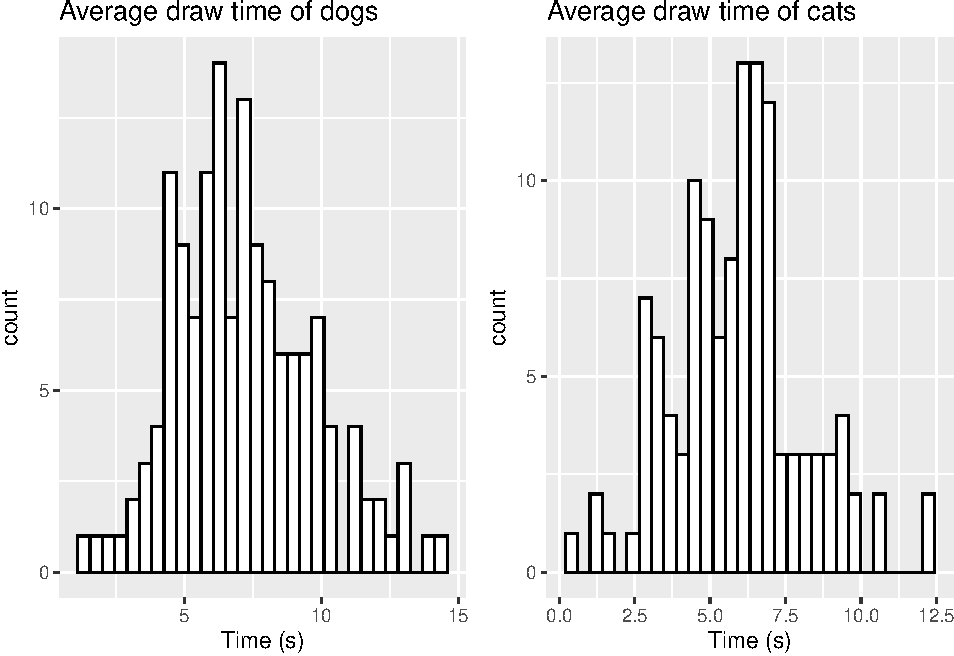
\includegraphics{bookdown-demo_files/figure-latex/histograms-1.pdf}

To create these histograms, the code above works in the following fashion:

\begin{itemize}
\tightlist
\item
  We first specify our data using \texttt{ggplot(data)}, where our data here is either group of samples.
\item
  To specify which variables we would like to select, we use the \texttt{aes()} argument. As we only have one sample of data in each case, we specify this using \texttt{x=data}.
\item
  We then generate the histogram using \texttt{geom\_histogram()}, where we can define the line colour using \texttt{color} and the filled colour of the bars using \texttt{fill}.
\item
  We can label our plot using the \texttt{labs} argument, where we can include a \texttt{title} and an \texttt{x} axis label
\end{itemize}

We can also alter the number of bins we use (\texttt{ggplot} will set a standard number of bins by default) using the \texttt{bins} argument. Let's alter the number of bins for the dog data to be 10

\begin{Shaded}
\begin{Highlighting}[]
\NormalTok{dog\_hist }\OtherTok{\textless{}{-}} \FunctionTok{ggplot}\NormalTok{(}\FunctionTok{data.frame}\NormalTok{(sample\_dog),}\FunctionTok{aes}\NormalTok{(}\AttributeTok{x=}\NormalTok{sample\_dog)) }\SpecialCharTok{+} \FunctionTok{geom\_histogram}\NormalTok{(}\AttributeTok{color=}\StringTok{"black"}\NormalTok{,}\AttributeTok{fill=}\StringTok{"white"}\NormalTok{,}\AttributeTok{bins=}\DecValTok{10}\NormalTok{) }\SpecialCharTok{+} 
  \FunctionTok{labs}\NormalTok{(}\AttributeTok{title=}\StringTok{"Average draw time of dogs"}\NormalTok{,}\AttributeTok{x=}\StringTok{"Time (s)"}\NormalTok{)}
\end{Highlighting}
\end{Shaded}

\hypertarget{setting-random-seeds-for-reproducability}{%
\subsection{Setting random seeds for reproducability}\label{setting-random-seeds-for-reproducability}}

When we randomly sample data each time in R, we will obtain a different sample than before. Let's run our previous code twice to see if there is any differences:

\begin{Shaded}
\begin{Highlighting}[]
\NormalTok{sample\_dog1 }\OtherTok{\textless{}{-}} \FunctionTok{rtruncnorm}\NormalTok{(}\AttributeTok{n=}\DecValTok{145}\NormalTok{, }\AttributeTok{a=}\DecValTok{0}\NormalTok{, }\AttributeTok{b=}\DecValTok{16}\NormalTok{, }\AttributeTok{mean=}\FloatTok{7.5}\NormalTok{, }\AttributeTok{sd=}\FloatTok{2.66}\NormalTok{)}
\NormalTok{sample\_dog2 }\OtherTok{\textless{}{-}} \FunctionTok{rtruncnorm}\NormalTok{(}\AttributeTok{n=}\DecValTok{145}\NormalTok{, }\AttributeTok{a=}\DecValTok{0}\NormalTok{, }\AttributeTok{b=}\DecValTok{16}\NormalTok{, }\AttributeTok{mean=}\FloatTok{7.5}\NormalTok{, }\AttributeTok{sd=}\FloatTok{2.66}\NormalTok{)}

\FunctionTok{summary}\NormalTok{(sample\_dog1)}
\end{Highlighting}
\end{Shaded}

\begin{verbatim}
##    Min. 1st Qu.  Median    Mean 3rd Qu.    Max. 
##  0.4464  5.7736  7.3936  7.5150  9.2837 13.4899
\end{verbatim}

\begin{Shaded}
\begin{Highlighting}[]
\FunctionTok{summary}\NormalTok{(sample\_dog2)}
\end{Highlighting}
\end{Shaded}

\begin{verbatim}
##    Min. 1st Qu.  Median    Mean 3rd Qu.    Max. 
##  0.2391  5.3456  7.5616  7.4537  9.2504 13.4568
\end{verbatim}

We see that both samples produce different summary statistics. This can cause difficulty when you are working on a specific problem and want to design questions around the specific characteristics of the data you have sampled the first time.

We can force R to use the same random number generation by using the \texttt{set.seed()} function. Here, we specify the seed from the random number generator we want to use each time we generate samples. This number can be any number you wish to choose! The example below highlights how this works:

\begin{Shaded}
\begin{Highlighting}[]
\FunctionTok{set.seed}\NormalTok{(}\DecValTok{2023}\NormalTok{)}
\NormalTok{sample\_dog1 }\OtherTok{\textless{}{-}} \FunctionTok{rtruncnorm}\NormalTok{(}\AttributeTok{n=}\DecValTok{145}\NormalTok{, }\AttributeTok{a=}\DecValTok{0}\NormalTok{, }\AttributeTok{b=}\DecValTok{16}\NormalTok{, }\AttributeTok{mean=}\FloatTok{7.5}\NormalTok{, }\AttributeTok{sd=}\FloatTok{2.66}\NormalTok{)}
\FunctionTok{set.seed}\NormalTok{(}\DecValTok{2023}\NormalTok{)}
\NormalTok{sample\_dog2 }\OtherTok{\textless{}{-}} \FunctionTok{rtruncnorm}\NormalTok{(}\AttributeTok{n=}\DecValTok{145}\NormalTok{, }\AttributeTok{a=}\DecValTok{0}\NormalTok{, }\AttributeTok{b=}\DecValTok{16}\NormalTok{, }\AttributeTok{mean=}\FloatTok{7.5}\NormalTok{, }\AttributeTok{sd=}\FloatTok{2.66}\NormalTok{)}

\FunctionTok{summary}\NormalTok{(sample\_dog1)}
\end{Highlighting}
\end{Shaded}

\begin{verbatim}
##    Min. 1st Qu.  Median    Mean 3rd Qu.    Max. 
##   2.006   6.316   7.545   7.798   9.365  14.776
\end{verbatim}

\begin{Shaded}
\begin{Highlighting}[]
\FunctionTok{summary}\NormalTok{(sample\_dog2)}
\end{Highlighting}
\end{Shaded}

\begin{verbatim}
##    Min. 1st Qu.  Median    Mean 3rd Qu.    Max. 
##   2.006   6.316   7.545   7.798   9.365  14.776
\end{verbatim}

Here, we see we can produce the same data as the first sample by setting the seed prior to sampling.

\hypertarget{manually-editing-data}{%
\subsection{Manually editing data}\label{manually-editing-data}}

If we take a sample of data and perhaps wish to add some additional variables to mimic the original data closer, this can easily be done in R. Let's take a sample for the dog data but lower our boundary to 14 and visualise

\begin{Shaded}
\begin{Highlighting}[]
\NormalTok{sample\_dog }\OtherTok{\textless{}{-}} \FunctionTok{rtruncnorm}\NormalTok{(}\AttributeTok{n=}\DecValTok{145}\NormalTok{, }\AttributeTok{a=}\DecValTok{0}\NormalTok{, }\AttributeTok{b=}\DecValTok{14}\NormalTok{, }\AttributeTok{mean=}\FloatTok{7.5}\NormalTok{, }\AttributeTok{sd=}\FloatTok{2.66}\NormalTok{)}

\FunctionTok{ggplot}\NormalTok{(}\FunctionTok{data.frame}\NormalTok{(sample\_dog),}\FunctionTok{aes}\NormalTok{(}\AttributeTok{x=}\NormalTok{sample\_dog)) }\SpecialCharTok{+} \FunctionTok{geom\_histogram}\NormalTok{(}\AttributeTok{color=}\StringTok{"black"}\NormalTok{,}\AttributeTok{fill=}\StringTok{"white"}\NormalTok{,}\AttributeTok{bins=}\DecValTok{12}\NormalTok{) }\SpecialCharTok{+} 
            \FunctionTok{labs}\NormalTok{(}\AttributeTok{title=}\StringTok{"Average draw time of dogs"}\NormalTok{,}\AttributeTok{x=}\StringTok{"Time (s)"}\NormalTok{)}
\end{Highlighting}
\end{Shaded}

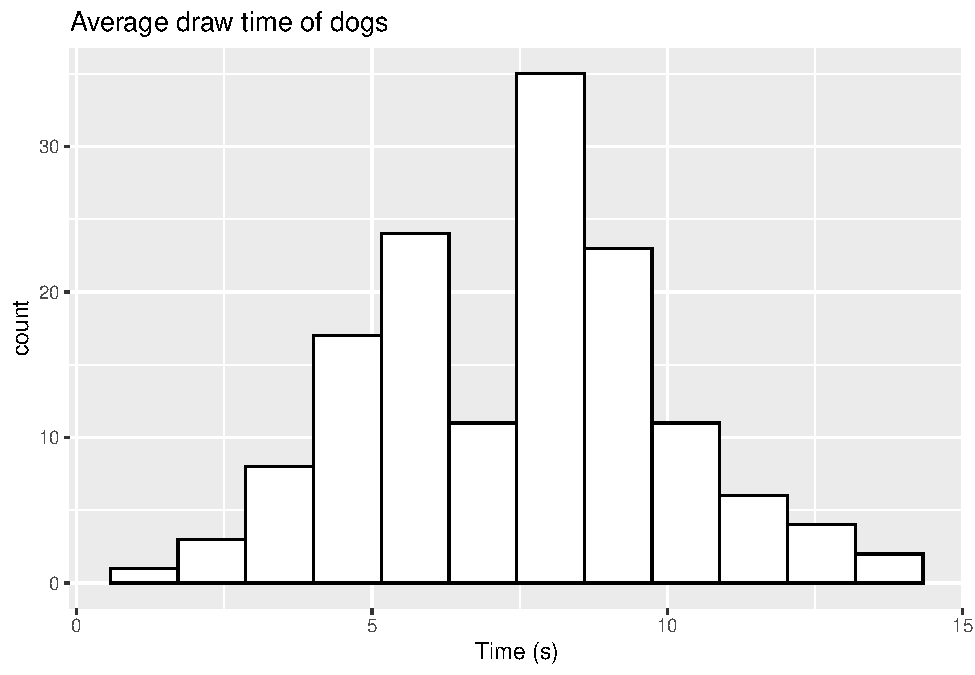
\includegraphics{bookdown-demo_files/figure-latex/lowsample-1.pdf}

When comparing this to the original data from the paper, we see that we do not observe the two outliers at 14.3 seconds and 15.2 seconds. We can manually add these values as follows:

\begin{Shaded}
\begin{Highlighting}[]
\NormalTok{sample\_dog }\OtherTok{\textless{}{-}} \FunctionTok{c}\NormalTok{(sample\_dog, }\FunctionTok{c}\NormalTok{(}\FloatTok{14.3}\NormalTok{,}\FloatTok{15.2}\NormalTok{))}

\FunctionTok{ggplot}\NormalTok{(}\FunctionTok{data.frame}\NormalTok{(sample\_dog),}\FunctionTok{aes}\NormalTok{(}\AttributeTok{x=}\NormalTok{sample\_dog)) }\SpecialCharTok{+} \FunctionTok{geom\_histogram}\NormalTok{(}\AttributeTok{color=}\StringTok{"black"}\NormalTok{,}\AttributeTok{fill=}\StringTok{"white"}\NormalTok{,}\AttributeTok{bins=}\DecValTok{12}\NormalTok{) }\SpecialCharTok{+} 
            \FunctionTok{labs}\NormalTok{(}\AttributeTok{title=}\StringTok{"Average draw time of dogs"}\NormalTok{,}\AttributeTok{x=}\StringTok{"Time (s)"}\NormalTok{)}
\end{Highlighting}
\end{Shaded}

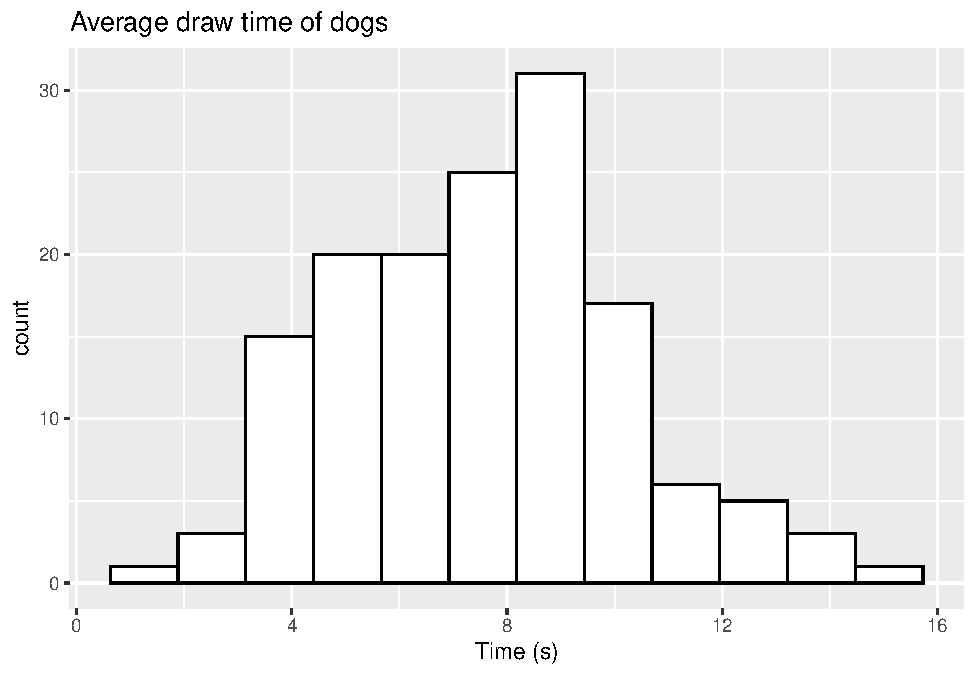
\includegraphics{bookdown-demo_files/figure-latex/modify-1.pdf}
We now observe the two additional values in the histogram. For a vector of data, we can easily add new values using the \texttt{c()} command. This can be done by specifying our original data first, and then including our additional variables in a new \texttt{c()} object. If we only wish to add one value, we do not need to use \texttt{c()}.

\hypertarget{sampling-from-different-distributions}{%
\subsection{Sampling from different distributions}\label{sampling-from-different-distributions}}

In this case, the data shown roughly takes the form of a Normal distribution. There are several cases where this may not be an appropriate distribution. R contains a full range of different distributions we can sample from. Some common choices are shown below:

\begin{itemize}
\tightlist
\item
  \texttt{rbinom()} - Sample from a Binomial distribution
\item
  \texttt{rchisq()} - Sample from a Chi-squared distribution
\item
  \texttt{rgamma()} - Sample from a Gamma distribution
\item
  \texttt{runif()} - Sample from a Uniform distribution
\item
  \texttt{rexp()} - Sample from an Exponential distribution
\end{itemize}

This list is not exhaustive, and R will contain libraries that will allow sampling from almost any known distribution.

\hypertarget{performing-a-mann-whitney-test}{%
\subsection{Performing a Mann-Whitney Test}\label{performing-a-mann-whitney-test}}

We can carry out a Mann-Whitney test in R as follows

\begin{Shaded}
\begin{Highlighting}[]
\NormalTok{sample\_dog }\OtherTok{\textless{}{-}} \FunctionTok{rtruncnorm}\NormalTok{(}\AttributeTok{n=}\DecValTok{145}\NormalTok{, }\AttributeTok{a=}\DecValTok{0}\NormalTok{, }\AttributeTok{b=}\DecValTok{16}\NormalTok{, }\AttributeTok{mean=}\FloatTok{7.5}\NormalTok{, }\AttributeTok{sd=}\FloatTok{2.66}\NormalTok{)}
\NormalTok{sample\_cat }\OtherTok{\textless{}{-}} \FunctionTok{rtruncnorm}\NormalTok{(}\AttributeTok{n=}\DecValTok{121}\NormalTok{, }\AttributeTok{a=}\DecValTok{0}\NormalTok{, }\AttributeTok{b=}\DecValTok{14}\NormalTok{, }\AttributeTok{mean=}\FloatTok{5.4}\NormalTok{, }\AttributeTok{sd=}\FloatTok{2.31}\NormalTok{)}

\NormalTok{mann\_whitney }\OtherTok{\textless{}{-}} \FunctionTok{wilcox.test}\NormalTok{(sample\_dog,sample\_cat)}
\NormalTok{mann\_whitney}
\end{Highlighting}
\end{Shaded}

\begin{verbatim}
## 
##  Wilcoxon rank sum test with continuity correction
## 
## data:  sample_dog and sample_cat
## W = 12823, p-value = 9.048e-11
## alternative hypothesis: true location shift is not equal to 0
\end{verbatim}

The output from this test gives us the rank sum \texttt{W} and a p-value which can be used for question creation

\hypertarget{performing-a-z-test}{%
\section{Performing a z-test}\label{performing-a-z-test}}

We can perform a two-sample z test in R using the \texttt{z.test} function from the \texttt{BSDA} package. We can carry out this test as follows:

\begin{Shaded}
\begin{Highlighting}[]
\FunctionTok{z.test}\NormalTok{(sample\_cat,sample\_dog,}\AttributeTok{sigma.x=}\FloatTok{2.307}\NormalTok{,}\AttributeTok{sigma.y=}\FloatTok{2.655}\NormalTok{)}
\end{Highlighting}
\end{Shaded}

\begin{verbatim}
## 
##  Two-sample z-Test
## 
## data:  sample_cat and sample_dog
## z = -6.7694, p-value = 1.293e-11
## alternative hypothesis: true difference in means is not equal to 0
## 95 percent confidence interval:
##  -2.656354 -1.463513
## sample estimates:
## mean of x mean of y 
##  5.308262  7.368196
\end{verbatim}

Here, we specify the sample standard deviation for cats and dogs respectively. The output from the test gives us the z-statistic, p-value and 95\% confidence interval.

\hypertarget{regression-example}{%
\chapter{Regression example}\label{regression-example}}

In this section we will introduce how to generate data for a linear model example using the linear model equation.

This example is based on the following question.

\hypertarget{question}{%
\section{Question}\label{question}}

A global ice cream company is interested in using linear regression to predict its ice cream waste (kg) based on the average temperatures of its store locations (\(^{\circ}\)C).

The estimated linear model is:

\[\hat{waste} = 591 - 10.65 \times temperature.\]

\begin{enumerate}
\def\labelenumi{\arabic{enumi}.}
\item
  What is the predicted waste for a store location whose average temperature is 18\(^{\circ}\)C?
\item
  The standard error for the slope coefficient is 0.38, which is associated with \(df=32\). Calculate a 95\% confidence interval for the slope parameter.
\item
  Suppose you performed a hypothesis test to test if average temperature is a significant predictor of ice cream waste. Working at a significance level of 5\%, would you expect the p-value of the hypothesis test to be:
\end{enumerate}

\hypertarget{radio_XPMJYNFZEM}{}
{Cannot tell with the information provided} {greater than 0.05} {less than 0.05}

\hypertarget{generating-our-data}{%
\section{Generating our data}\label{generating-our-data}}

In order to fit this linear model we need to generate two variables:

\begin{itemize}
\tightlist
\item
  Response variable (\(y\)): \(waste\) and
\item
  Explanatory variable (\(x\)): \(temperature\).
\end{itemize}

Crucially, these variables need to be associated with each other as shown in the linear model equation.

Let's start by generating our x-variable, \(temperature\). We will use a Normal distribution to do this since our variable is continuous.

\begin{Shaded}
\begin{Highlighting}[]
\NormalTok{temp}\OtherTok{\textless{}{-}}\FunctionTok{rnorm}\NormalTok{(}\AttributeTok{n=}\DecValTok{34}\NormalTok{, }\AttributeTok{mean=}\DecValTok{12}\NormalTok{, }\AttributeTok{sd=}\DecValTok{4}\NormalTok{)}
\end{Highlighting}
\end{Shaded}

The parameters required are defined as follows:

\begin{itemize}
\tightlist
\item
  \texttt{n} - the number of samples we wish to draw. In our question \(df=32\), so \(n=34\) (since for a simple linear model \(df=n-2\)).
\item
  \texttt{mean} - the mean temperature which our data will be centered on. Pick something sensible here, we have gone for \(12^{\circ}\)C.
\item
  \texttt{sd} - the standard deviation for \(temperature\). Again go for something that seems sensible (high enough to show some variability, but not too high that the values at the extreme are no longer sensible). This can take a bit of trial and error.
\end{itemize}

  \bibliography{book.bib,packages.bib}

\end{document}
